\chapter{Conception détaillée des données}
\label{chap:donnees}

Le défi central de BCaaS est de modéliser des entités métier hétérogènes (médecin, livre,
appartement, produit agricole, etc.) avec un schéma de données unique et générique. Nous
adoptons une modélisation Merise (MCD, MLD) complétée par un diagramme de classes UML.

%\section{Modèle Conceptuel de Données (MCD)}

%\figplaceholder{Modèle Conceptuel de Données (Merise) %: entités TENANT, USER, ACTOR,
%PORTFOLIO, BUSINESS, BUSINESS\_RULE, %SERVICE\_CATALOGUE, RESOURCE, MEDIA, SERVICE\_REQUEST,
%INVOICE, MESSAGE, NOTIFICATION, AUDIT\_EVENT et leurs %associations avec cardinalités.}{7.5cm}
%\captionof{figure}{Modèle Conceptuel de Données de %BCaaS}
%\label{fig:mcd}

\section{Dictionnaire des entités}

Le domaine compte quinze entités (plus l'énumération \texttt{SupportedCurrency} et la table
de jonction \texttt{portfolio\_businesses}). Le tableau~\ref{tab:entites} en récapitule la
structure.

\begin{table}[H]
\centering
\caption{Entités du modèle de données --- Business Core}
\label{tab:entites}
\renewcommand{\arraystretch}{1.25}\scriptsize
\begin{tabularx}{\linewidth}{L{2.5cm} X}
\toprule
\textbf{Entité (table)} & \textbf{Attributs principaux et relations} \\
\midrule
\texttt{Tenant} (tenants) & \texttt{id}, \texttt{name} (unique), \texttt{domain}, \texttt{description}, \texttt{isActive}, \texttt{createdAt}. Racine du multi-tenant. \\
\texttt{User} (users) & \texttt{id}, \texttt{firstName}, \texttt{lastName}, \texttt{email} (unique), \texttt{password}, \texttt{phone}, \texttt{country}, \texttt{roles} (Set), \texttt{isActive}, \texttt{createdAt} ; \texttt{ManyToOne} $\to$ Tenant. \\
\texttt{Actor} (actors) & \texttt{id}, \texttt{role}, \texttt{bio}, \texttt{isActive}, \texttt{createdAt} ; \texttt{ManyToOne} $\to$ User. \\
\texttt{Business} (businesses) & \texttt{id}, \texttt{name}, \texttt{domain}, \texttt{description}, \texttt{typeOfInvolvedActors}, \texttt{requiredJobProfile}, \texttt{createdAt} ; \texttt{ManyToOne} $\to$ Tenant. \\
\texttt{BusinessRule} (business\_rules) & \texttt{id}, \texttt{ruleKey}, \texttt{ruleValue}, \texttt{description}, \texttt{createdAt} ; \texttt{ManyToOne} $\to$ Business. \\
\texttt{ServiceCatalogue} (service\_catalogues) & \texttt{id}, \texttt{name}, \texttt{description}, \texttt{basePrice}, \texttt{currency}, \texttt{isAvailable}, \texttt{createdAt} ; \texttt{ManyToOne} $\to$ Business. \\
\texttt{Resource} (resources) & \texttt{id}, \texttt{name}, \texttt{type}, \texttt{quantity}, \texttt{description}, \texttt{createdAt} ; \texttt{ManyToOne} $\to$ Business. \\
\texttt{Media} (media) & \texttt{id}, \texttt{type}, \texttt{url}, \texttt{label}, \texttt{createdAt} ; \texttt{ManyToOne} $\to$ Business. \\
\texttt{Portfolio} (portfolios) & \texttt{id}, \texttt{title}, \texttt{description}, \texttt{createdAt} ; \texttt{OneToOne} $\to$ Actor ; \texttt{ManyToMany} $\to$ Business (\texttt{portfolio\_businesses}). \\
\texttt{ServiceRequest} (service\_requests) & \texttt{id}, \texttt{serviceName}, \texttt{description}, \texttt{status}, \texttt{traceId}, \texttt{correlationId}, 5 timestamps ; \texttt{ManyToOne} $\to$ Tenant, consumer Actor, provider Actor, ServiceCatalogue. \\
\texttt{Invoice} (invoices) & \texttt{id}, \texttt{amount}, \texttt{currency}, \texttt{status}, \texttt{issuedAt}, \texttt{paidAt} ; \texttt{OneToOne} $\to$ ServiceRequest (unique). \\
\texttt{Message} (messages) & \texttt{id}, \texttt{content}, \texttt{isRead}, \texttt{createdAt} ; \texttt{ManyToOne} $\to$ ServiceRequest, sender Actor, Tenant. \\
\texttt{Notification} (notifications) & \texttt{id}, \texttt{title}, \texttt{message}, \texttt{isRead}, \texttt{createdAt} ; \texttt{ManyToOne} $\to$ User, Tenant. \\
\texttt{AuditEvent} (audit\_events) & \texttt{id}, \texttt{entityType}, \texttt{action}, \texttt{previousStatus}, \texttt{newStatus}, \texttt{ipAddress}, \texttt{userAgent}, \texttt{metadata} (JSON), \texttt{tenantId}, \texttt{actorId}, \texttt{entityId}, \texttt{traceId} (UUID bruts). \\
\bottomrule
\end{tabularx}
\end{table}

\noindent Toutes les entités utilisent une génération d'identifiant
\texttt{GenerationType.UUID} et un \texttt{@PrePersist} initialisant \texttt{createdAt}.

\section{Modèle Logique de Données (MLD)}

Le passage au modèle relationnel traduit les associations par des clés étrangères. En
particulier, l'isolation multi-tenant repose sur une colonne \texttt{tenant\_id} (UUID,
clé étrangère vers \texttt{tenants}) portée par les tables racines du tenant
(\texttt{users}, \texttt{businesses}, \texttt{service\_requests}, \texttt{messages},
\texttt{notifications}, \texttt{audit\_events}). L'entité \texttt{Actor} n'a pas de
\texttt{tenant\_id} direct : elle hérite du contexte tenant via son \texttt{User}.

%\figplaceholder{Modèle Logique de Données (schéma %relationnel) : tables et clés étrangères,
%mise en évidence des colonnes \texttt{tenant\_id} et %des contraintes d'unicité.}{6.5cm}
%\captionof{figure}{Modèle Logique de Données de BCaaS}
%\label{fig:mld}

\begin{table}[h]
\centering
\caption{Entités du modèle de données – Business Core}
\label{tab:entites_business_core}
\begin{tabular}{|p{4cm}|p{12cm}|}
\hline
\textbf{Table} & \textbf{Attributes} \\
\hline
tenant & id\_Tenant, Name, IsActive, CreatedAt \\
\hline
user & Id\_User, FirstName, LastName, Email, Gender, Password, IsActive, Country, Phone, CreatedAt, \#id\_Tenant \\
\hline
actor & Id\_Actor, NomProfessionnel, Speciality, bio, CreatedAt, Role, \#Id\_User \\
\hline
formation & Id\_Formation, NomFormation, Description, Type\_Formation, Niveau \\
\hline
media & Id\_Media, Type, Url, Label, CreatedAt, \#Id\_Business \\
\hline
business & Id\_Business, NameBusiness, Domain, Type\_of\_InvolvedActors, RequiredJobProfile, CreatedAt \\
\hline
business\_rule & Id\_BusinessRule, RuleKey, RuleValue, Description, CreatedAt \\
\hline
ressource & Id\_Resource, NameRes, Type, Quantity, Description, CreatedAt, Disponibilité \\
\hline
service\_catalogue & Id\_SerCatalogue, NameSerCatalogue, Description, Currency, IsAvailable, CreatedAt \\
\hline
portfolio & Id\_Portfolio, title, Description, Status, \#Id\_Business \\
\hline
service\_request & Id\_ServiceRequest, TraceId, ServiceName, Description, Status, \#Id\_Actor, \#Id\_Portfolio \\
\hline
message & id\_Message, content, isRead, createdAt, \#Id\_ServiceRequest \\
\hline
notification & id\_Notification, title, message, isRead, createdAt, \#Id\_ServiceRequest \\
\hline
invoice & id\_Invoice, Amount, Currency, Status, UsedAt, PaidAt, IssueAt, \#Id\_ServiceRequest \\
\hline
\end{tabular}
\end{table}

\section{Diagramme de classes métier}

\begin{figure}[H]
    \centering
    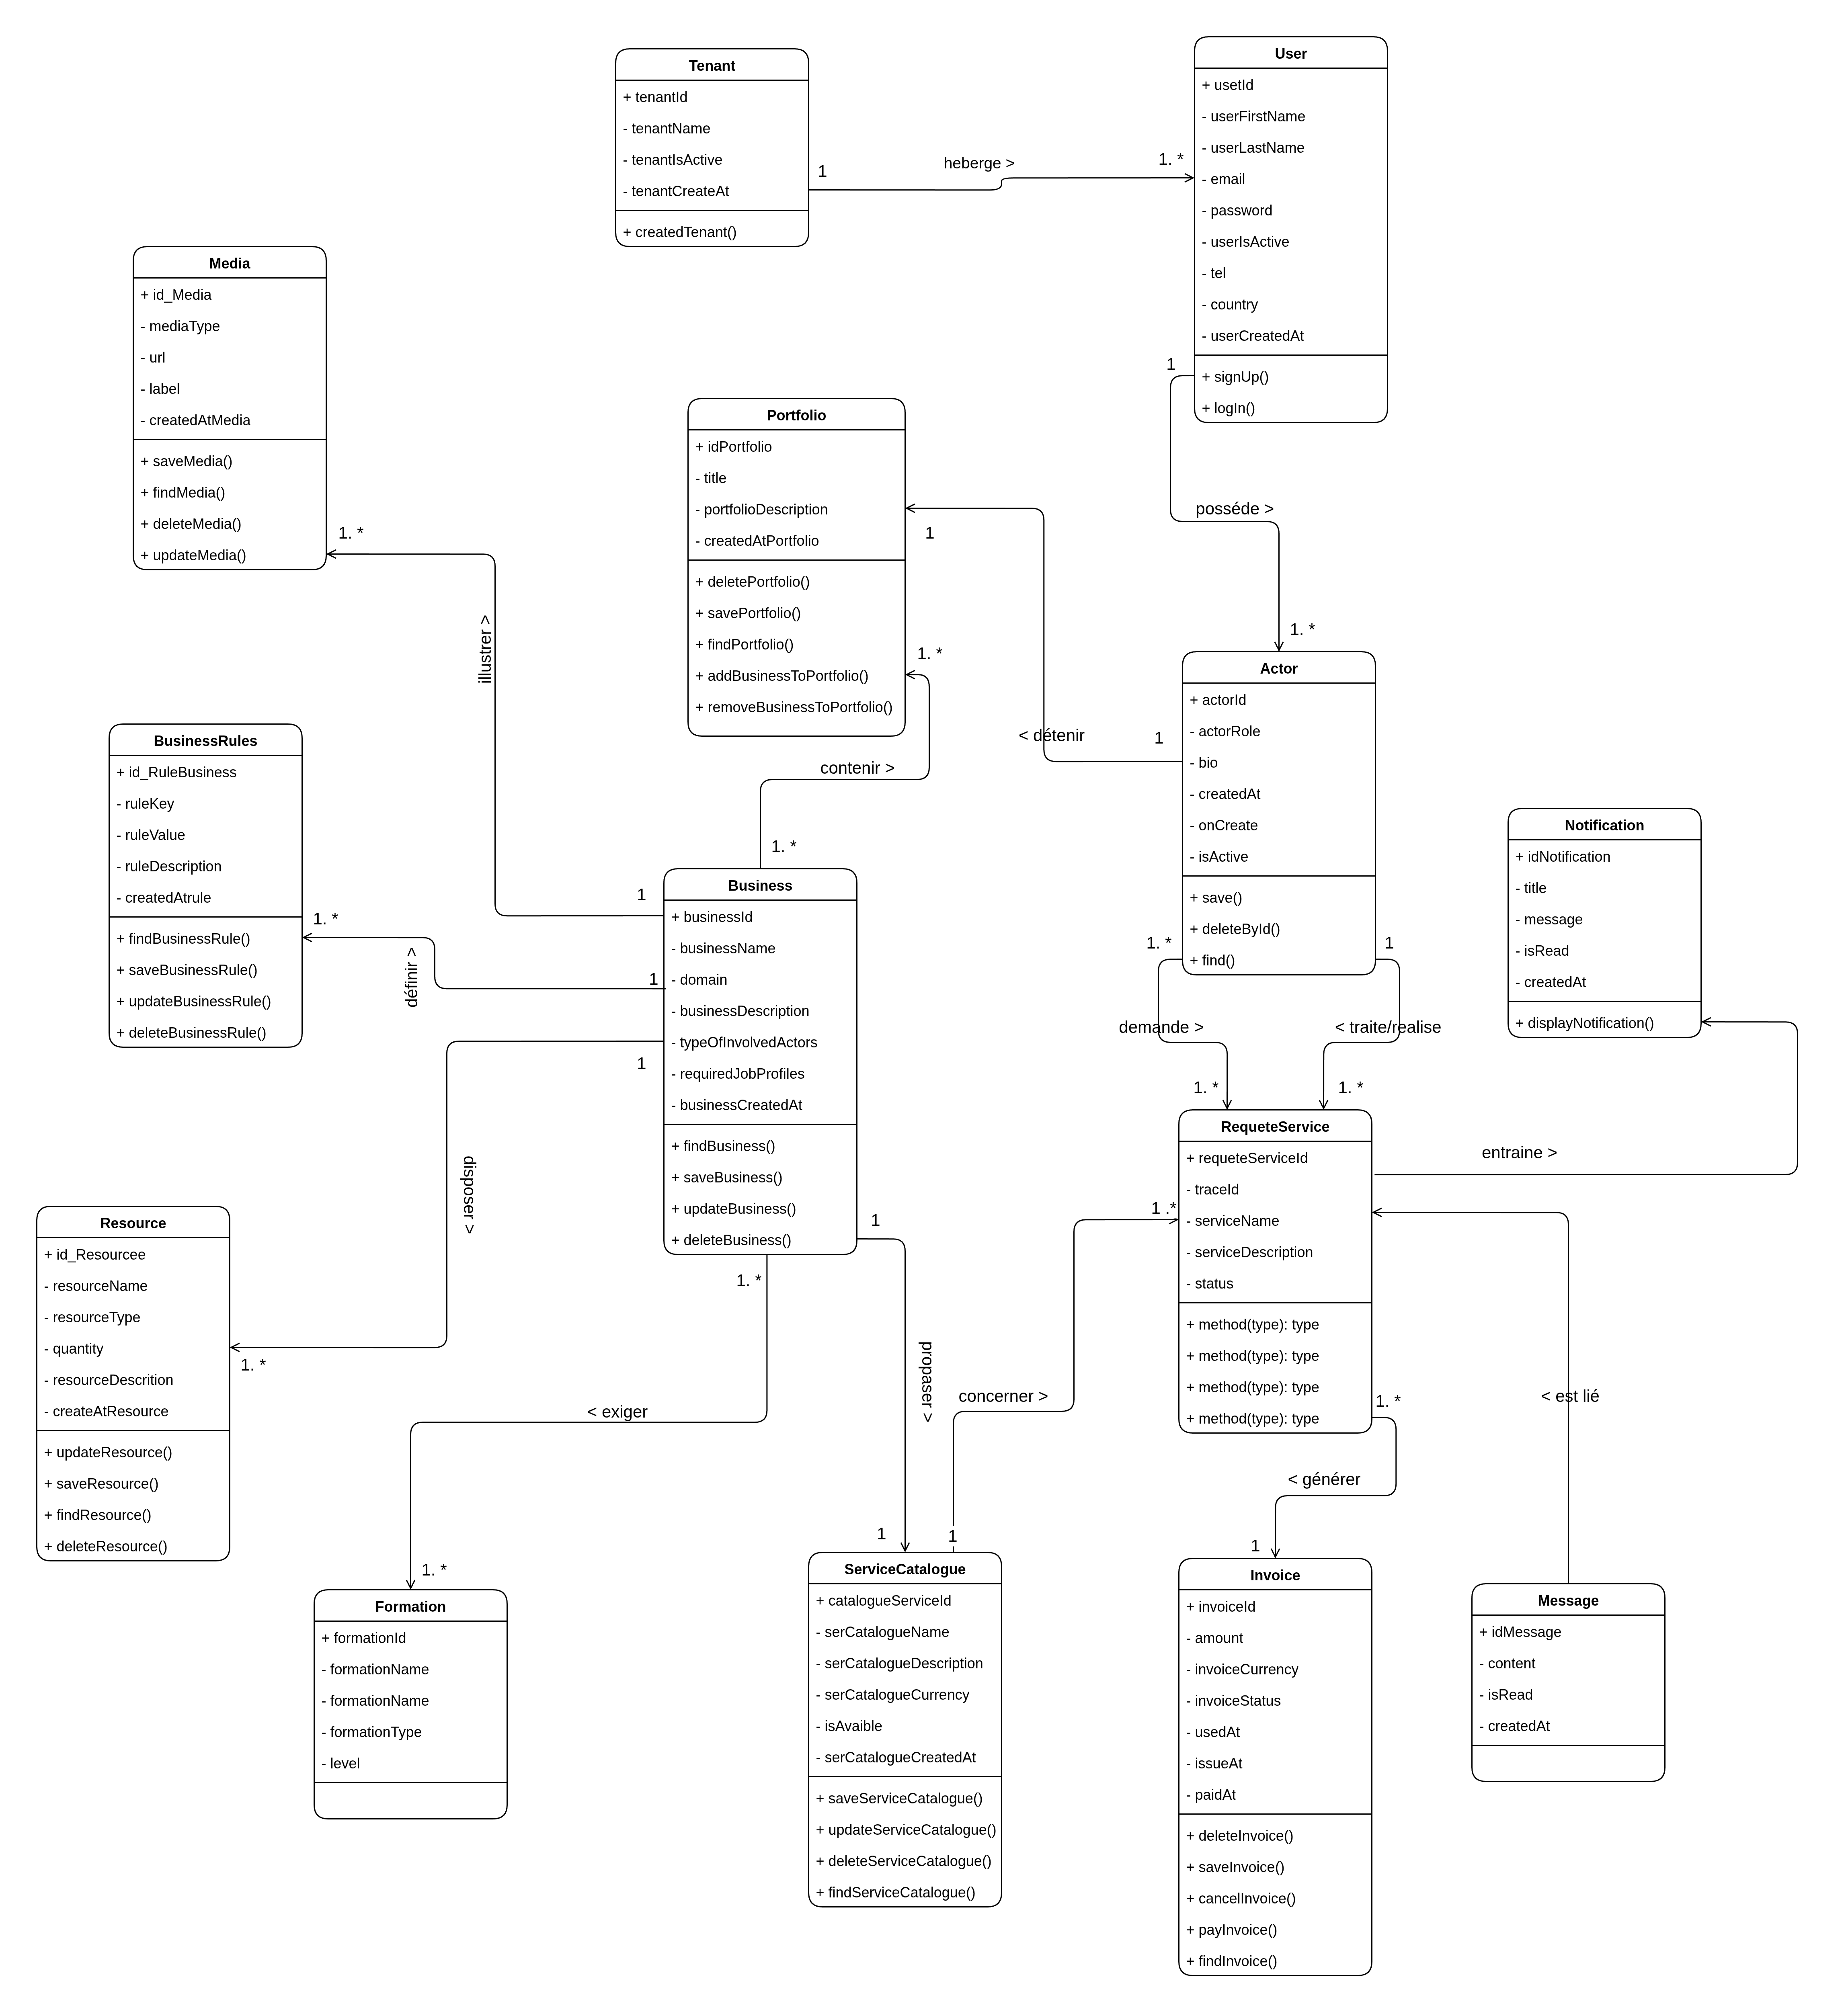
\includegraphics[width=0.8\linewidth]{chapitres/CLASSES (2) (1).drawio.png}
    \captionof{figure}{Diagramme de classes métier de BCaaS}
    \label{fig:placeholder}
\end{figure}
\label{fig:classes}

\section{Contraintes d'intégrité}

Le tableau~\ref{tab:integrite} liste les principales contraintes d'intégrité
référentielle et d'unicité.

\begin{table}[H]
\centering
\caption{Principales contraintes d'intégrité}
\label{tab:integrite}
\renewcommand{\arraystretch}{1.25}\footnotesize
\begin{tabularx}{\linewidth}{L{4cm} L{2.4cm} X}
\toprule
\textbf{Table} & \textbf{Type} & \textbf{Description} \\
\midrule
tenants            & Unique      & Nom de tenant unique \\
users              & Unique      & Email unique \\
users              & FK          & \texttt{tenant\_id} $\to$ tenants \\
portfolios         & Unique + FK & Un portfolio par acteur \\
service\_requests  & FK          & consumer, provider, catalogue, tenant existants \\
invoices           & Unique + FK & Une facture par demande de service \\
messages, notifications, audit\_events & FK (NOT NULL) & \texttt{tenant\_id} obligatoire \\
\bottomrule
\end{tabularx}
\end{table}

\section{Machines à états}

Deux entités portent une machine à états explicite. La \texttt{ServiceRequest} suit le
cycle \texttt{PENDING} $\to$ \texttt{ACCEPTED} $\to$ \texttt{IN\_PROGRESS} $\to$
\texttt{FULFILLED}, avec \texttt{CANCELLED} accessible depuis tout état non terminal ;
chaque transition horodate un champ dédié (\texttt{requestedAt}, \texttt{acceptedAt},
\texttt{startedAt}, \texttt{fulfilledAt}, \texttt{cancelledAt}). La transition
\texttt{fulfill} déclenche la génération automatique de l'\texttt{Invoice}. La facture
suit quant à elle \texttt{PENDING} $\to$ \texttt{PAID} ou \texttt{CANCELLED}.

% \figplaceholder{Diagrammes d'états-transitions UML : (a) ServiceRequest
% (PENDING/ACCEPTED/IN\_PROGRESS/FULFILLED/CANCELLED) ; (b) Invoice (PENDING/PAID/CANCELLED).}{5.5cm}

% \begin{figure}[H]
%   \centering
%   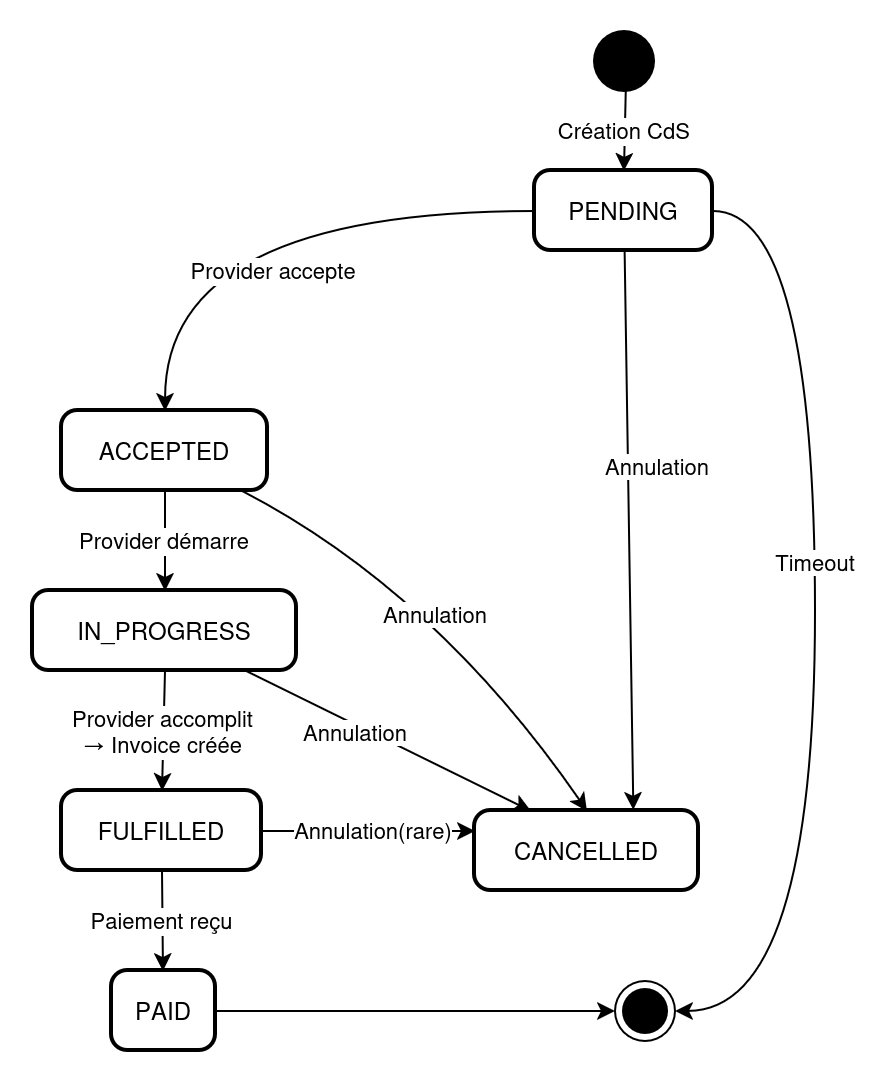
\includegraphics[width=0.6\textwidth]{figures/diagrammes/ETAT_SERVICE_REQUEST.drawio.png}
%   \caption{Machines à états de \texttt{ServiceRequest}.}
%   \label{fig:etatsr}
% \end{figure} 

% \begin{figure}[H]
%   \centering
%   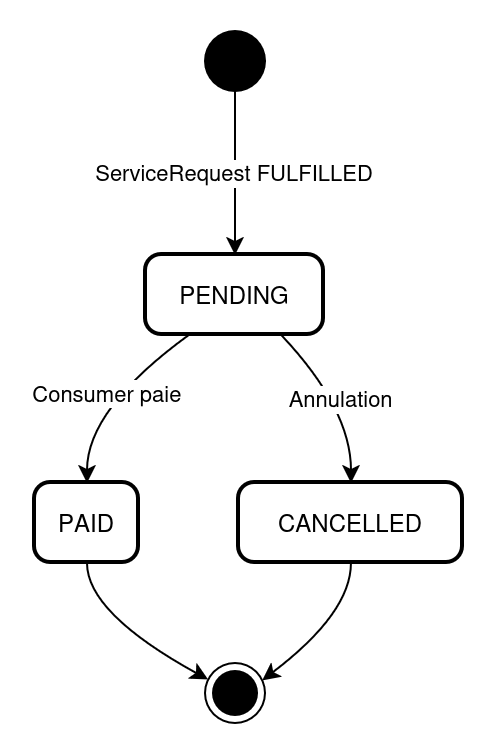
\includegraphics[width=0.4\textwidth]{figures/diagrammes/ETAT_INVOICE.drawio.png}
%   \caption{Machines à états de \texttt{INVOICE}.}
%   \label{fig:etatinvoice}
% \end{figure}

\begin{figure}[H]
  \centering
  \begin{minipage}{0.55\textwidth}
    \centering
    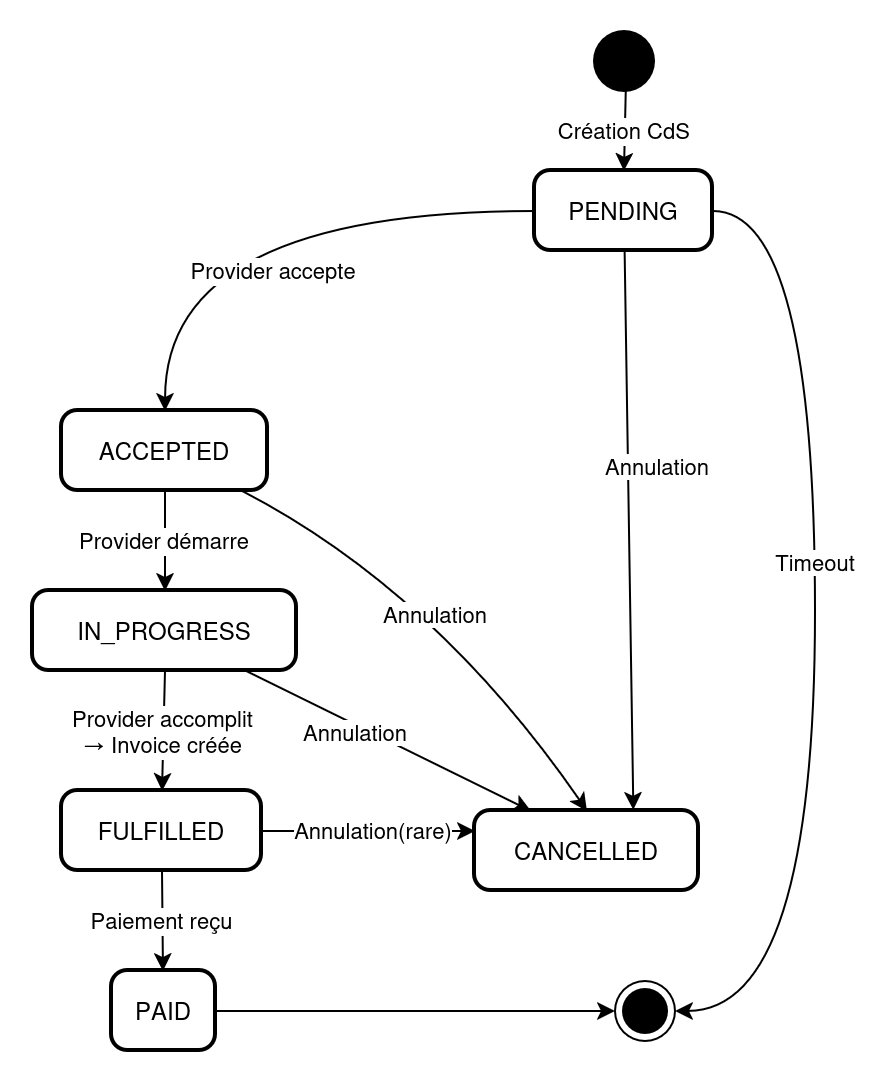
\includegraphics[width=\textwidth]{figures/diagrammes/ETAT_SERVICE_REQUEST.drawio.png}
    \caption{Machine à états de \texttt{ServiceRequest}}
    \label{fig:etatsr}
  \end{minipage}
  \hfill
  \begin{minipage}{0.38\textwidth}
    \centering
    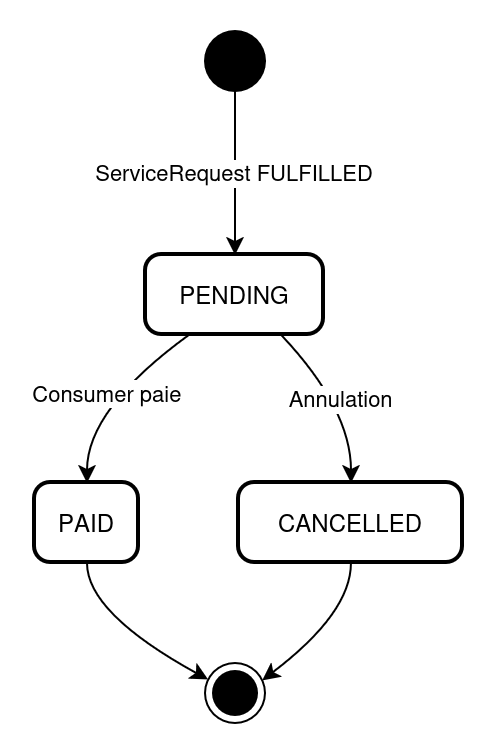
\includegraphics[width=\textwidth]{figures/diagrammes/ETAT_INVOICE.drawio.png}
    \caption{Machine à états de \texttt{Invoice}}
    \label{fig:etatinvoice}
  \end{minipage}
\end{figure}